\documentclass[11pt]{article}
\usepackage[T1,T2A]{fontenc}
\usepackage[utf8]{inputenc}
\usepackage[english,russian]{babel}
\usepackage{graphicx}
\usepackage{amsmath}
\graphicspath {{img/}}
\title{\textbf{Лабораторная работа №3\\<<Исследование устройств амплитудного преобразования сигналов в системах передачи информации>>}}
\author{Матяш А.А., ККСО-01-19}
\addtolength{\topmargin}{-3cm}
\addtolength{\textheight}{3cm}
\date{}
\begin{document}
\maketitle
\thispagestyle{empty}
\textbf{Цель работы:} ознакомление с устройством, работой амплитудных 
модуляторов и демодуляторов сигналов и приобретение практических навыков 
моделирования этих устройств.

\section{Схема №1: исследование АМ сигналов}
\subsection{Перечень элементов, использованных в схемах, с
их краткими характеристиками}
\begin{itemize}
    \item[-] Источник переменного тока (3.54 В, 200 Гц)
    \item[-] Четырехканальный осциллограф
    \item[-] Источник одночастотной амплитудной модуляции (5 В, 1000/200 Гц) 2 шт.
    \item[-] Анализатор спектра 
    \item[-] Ключ
\end{itemize}


\subsection{Копии окон схемных файлов с позиционными обозначениями}
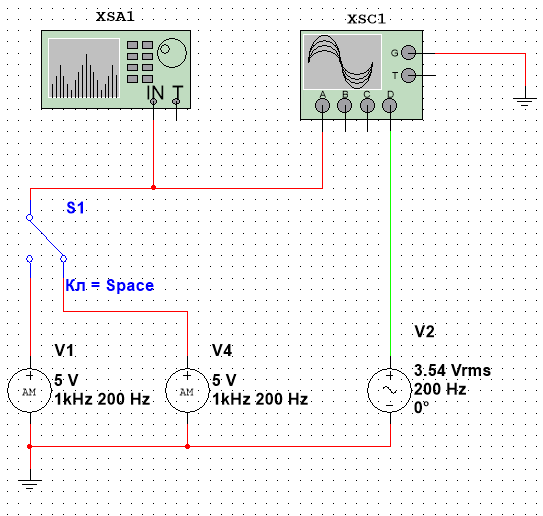
\includegraphics[width=1\linewidth]{img/first.png}
\begin{center}
    Рис.1 Схема исследования АМ сигналов
\end{center}

\subsection{Результаты расчетов и измерений приборами}
\begin{center}
    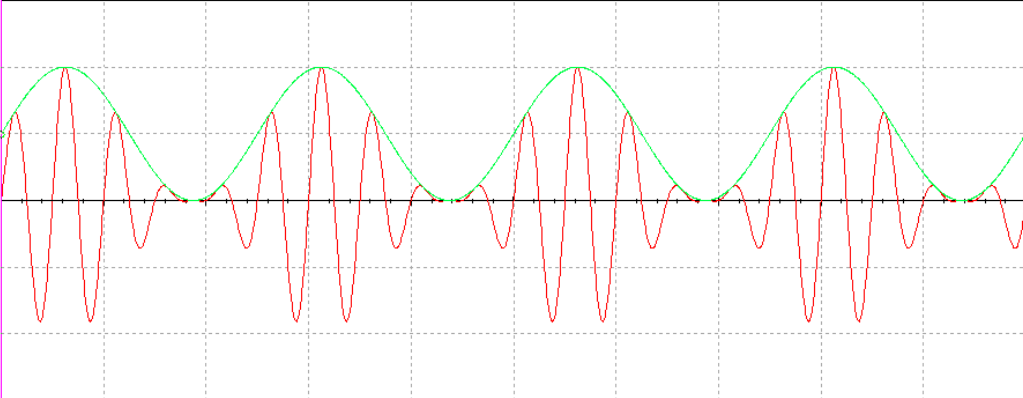
\includegraphics[width=1\linewidth]{img/first1.png}
        Рис.2 Показания осциллографа при первом положении ключа.
\end{center}

\begin{center}
    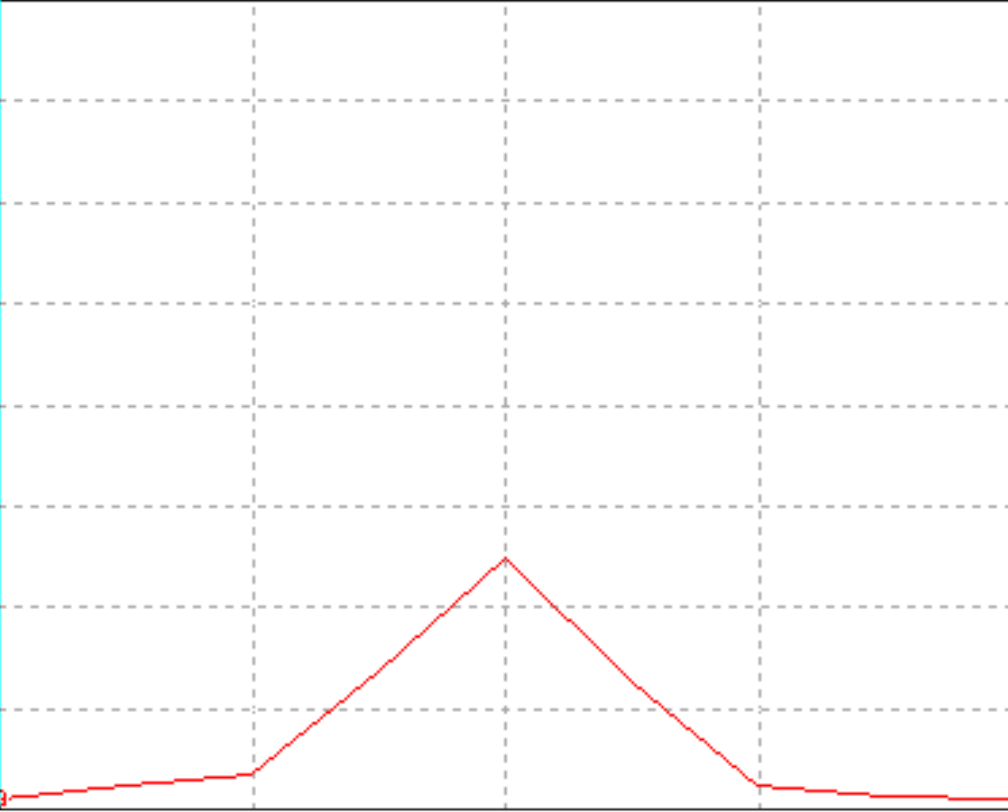
\includegraphics[scale=0.25]{img/first2.png}\\
        Рис.3 Показания анализатора спектра при первом положении ключа.
\end{center}


\begin{center}
    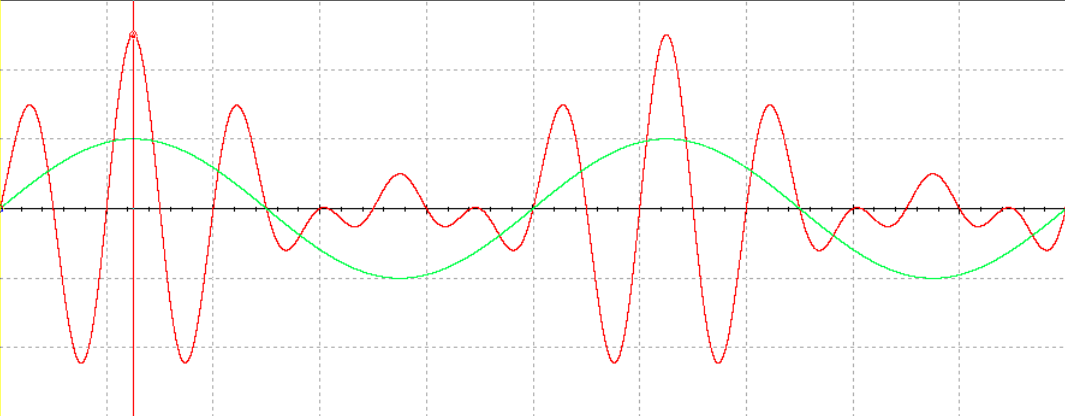
\includegraphics[width=1\linewidth]{img/first3.png}
        Рис.4 Показания осциллографа при втором положении ключа.
\end{center}

По данным показаниям можем определить коэффициент амплитудной модуляции. Вычислим этот коэффициент по второй осциллограмме:
\\
$$
M = \frac{{A_{max}+A_{min}}}{A_{max}-A_{min}} = \frac{{12.42+2.48}}{12.42-2.48}=1.4989\approx 1.5\\
$$
\\
Полученное нами значение примерно равно теоретическому значению.


\newpage
\section{Схема №2: Модель амплитудной демодуляции}
\subsection{Перечень элементов, использованных в схемах, с
их краткими характеристиками}
\begin{itemize}
    \item[-] Источник переменного тока (0.7 В, 10 кГц)
    \item[-] Четырехканальный осциллограф
    \item[-] Умножитель 2 шт.
    \item[-] Конденсатор (2мкФ)
    \item[-] Резистор (100 Ом)
\end{itemize}


\subsection{Копии окон схемных файлов с позиционными обозначениями}
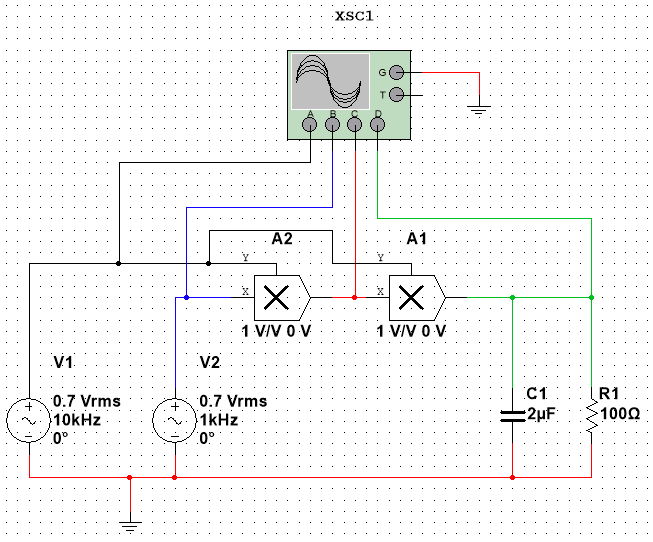
\includegraphics[width=1\linewidth]{img/second.png}
\begin{center}
    Рис.5 Схема амплитудного модулятора и демодулятора.
\end{center}

\subsection{Результаты расчетов и измерений приборами}
\begin{center}
    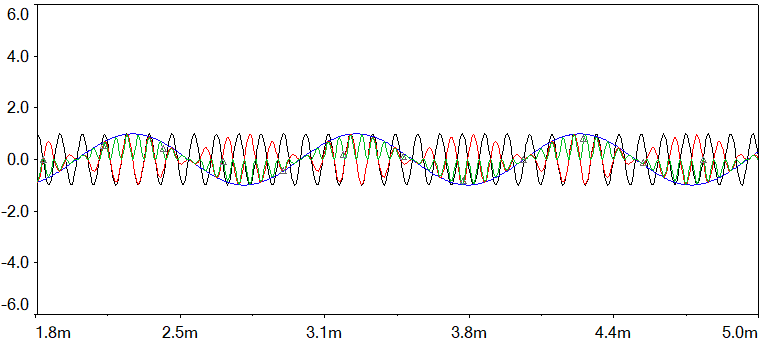
\includegraphics[width=1\linewidth]{img/second1.png}
        Рис.6 Показания осциллографа.
\end{center}
 
\newpage
\section{ Схема №3: модель системы передачи информации с амплитудной манипуляцией}
\subsection{Перечень элементов, использованных в схемах, с
их краткими характеристиками}
\begin{itemize}    
    \item[-] Источник переменного тока (5 В, 50 кГц)
    \item[-] Генератор слов
    \item[-] Логический анализатор
    \item[-] 8-битный ЦАП
    \item[-] Конденсатор 2мкФ
    \item[-] Резистор 100 Ом
    \item[-] Умножитель 2 шт.    
    \item[-] Четырехканальный осциллограф
    \item[-] Гистерезис по напряжению
\end{itemize}

\subsection{Копии окон схемных файлов с позиционными обозначениями}
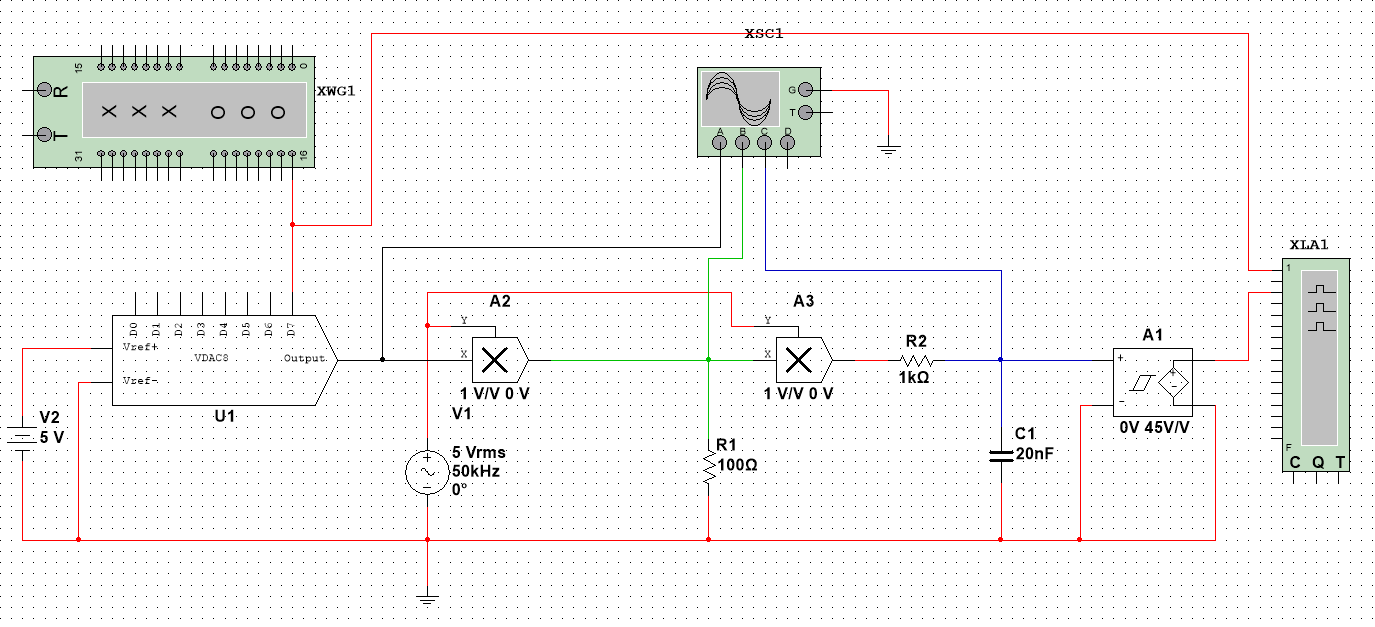
\includegraphics[width=1\linewidth]{img/third.png}
\begin{center}
    Рис.7 Схема системы передачи информации с амплитудной манипуляцией.
\end{center}

\subsection{Результаты расчетов и измерений приборами}
\begin{center}
    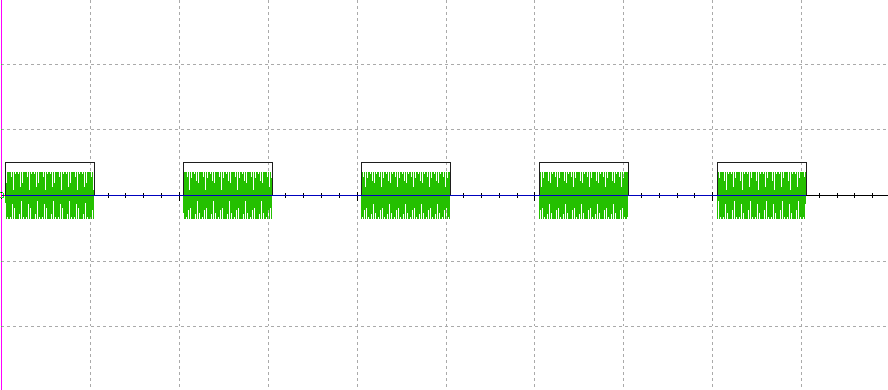
\includegraphics[width=1\linewidth]{img/third1.png}
        Рис.8 Показания осциллографа при 1 кГц.
\end{center}

\begin{center}
    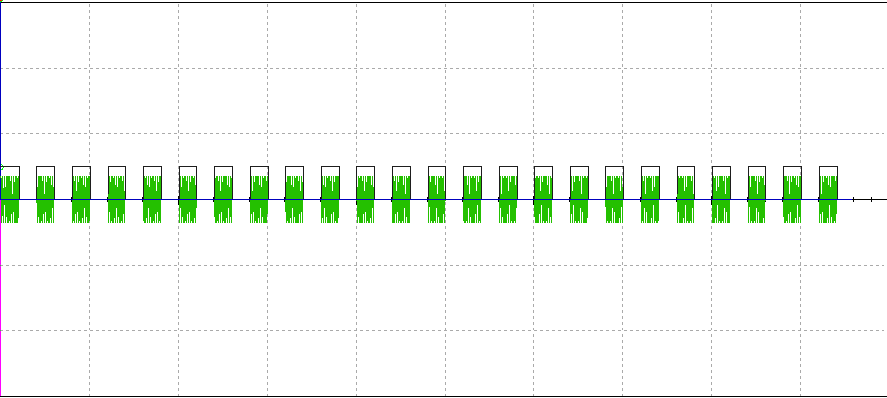
\includegraphics[width=1\linewidth]{img/third2.png}
        Рис.9 Показания осциллографа при 5 кГц.
\end{center}

\begin{center}
    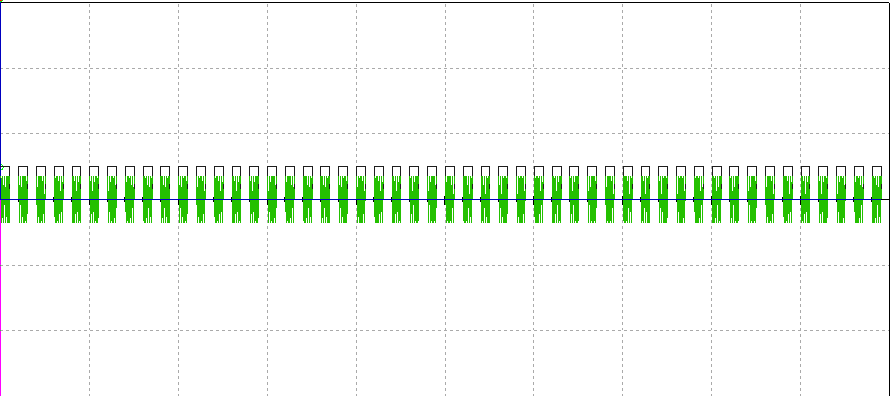
\includegraphics[width=1\linewidth]{img/third3.png}
        Рис.10 Показания осциллографа при 10 кГц.
\end{center}


\textbf{Вывод:} в ходе выполнения лабораторной работы мы изучили принцип передачи двоичных данных по сети связи, а также принципы работы и построения частотного модулятора и демодулятора.
\end{document}
